\documentclass[a4paper, 10pt, ]{article}

\usepackage[slovak]{babel}

% ------------------------------

\usepackage[utf8]{inputenc}
\usepackage[T1]{fontenc}

\usepackage[left=4cm,
            right=4cm,
            top=2.1cm,
            bottom=2.6cm,
            footskip=7.5mm,
            twoside,
            marginparwidth=3.0cm,
            %showframe,
            ]{geometry}

\usepackage{graphicx}
\usepackage[dvipsnames]{xcolor}
% https://en.wikibooks.org/wiki/LaTeX/Colors

% ------------------------------

\usepackage{lmodern}

\usepackage[tt={oldstyle=false,proportional=true,monowidth}]{cfr-lm}
% https://mirror.szerverem.hu/ctan/fonts/cfr-lm/doc/cfr-lm.pdf

% ------------------------------

\usepackage{amsmath}
\usepackage{amssymb}
\usepackage{amsthm}

\usepackage{booktabs}
\usepackage{multirow}
\usepackage{array}
\usepackage{dcolumn}

\usepackage{natbib}

% ------------------------------

\hyphenpenalty=6000
\tolerance=1000

\def\naT{\mathsf{T}}

% ------------------------------

\makeatletter

    \def\@seccntformat#1{\protect\makebox[0pt][r]{\csname the#1\endcsname\hspace{4mm}}}

    \def\cleardoublepage{\clearpage\if@twoside \ifodd\c@page\else
    \hbox{}
    \vspace*{\fill}
    \begin{center}
    \phantom{}
    \end{center}
    \vspace{\fill}
    \thispagestyle{empty}
    \newpage
    \if@twocolumn\hbox{}\newpage\fi\fi\fi}

    \newcommand\figcaption{\def\@captype{figure}\caption}
    \newcommand\tabcaption{\def\@captype{table}\caption}

\makeatother

% ------------------------------

\usepackage{fancyhdr}
\fancypagestyle{plain}{%
\fancyhf{} % clear all header and footer fields
% \fancyfoot[C]{\sffamily {\bfseries \thepage}\ | {\scriptsize\oznacenieCasti}}
\fancyfoot[C]{\sffamily {\bfseries \thepage}{\color{Gray}\scriptsize$\,$z$\,$\pageref{LastPage}}\ | 
\includegraphics[height=5pt]{../../COMMONFILES/KUT_logo_v0.1.pdf}{\scriptsize\KUTporadoveCislo}}
\renewcommand{\headrulewidth}{0pt}
\renewcommand{\footrulewidth}{0pt}}
\pagestyle{plain}

% ------------------------------

\usepackage{titlesec}
\titleformat{\paragraph}[hang]{\sffamily  \bfseries}{}{0pt}{}
\titlespacing*{\paragraph}{0mm}{3mm}{1mm}
\titlespacing*{\subparagraph}{0mm}{3mm}{1mm}

\titleformat*{\section}{\sffamily\Large\bfseries}
\titleformat*{\subsection}{\sffamily\large\bfseries}
\titleformat*{\subsubsection}{\sffamily\normalsize\bfseries}


% ------------------------------

\PassOptionsToPackage{hyphens}{url}
\usepackage[pdfauthor={},
            pdftitle={},
            pdfsubject={},
            pdfkeywords={},
            % hidelinks,
            colorlinks=false,
            breaklinks,
            ]{hyperref}


% ------------------------------

\graphicspath{%
{../fig_standalone/}%
{../../PY/fig/}%
{../../ML/fig/}%
{./fig/}%
}

% ------------------------------

\usepackage{enumitem}

\usepackage{lettrine}

% ------------------------------

\usepackage{lastpage}

\usepackage{microtype}

% ------------------------------

\usepackage{algorithm}
\usepackage[noend]{algpseudocode}
\makeatletter
\renewcommand{\ALG@name}{Algoritmus}
\makeatother
\usepackage{amsmath}
\usepackage{bbold}
\usepackage{calc}
\usepackage{dsfont}
\usepackage{mathtools}
\usepackage{tabto}


\newcommand{\mr}[1]{\mathrm{#1}}
\newcommand{\bs}[1]{\boldsymbol{#1}}
\newcommand{\bm}[1]{\mathbf{#1}}

\newcommand{\diff}[2]{\frac{\Delta #1}{\Delta #2}}
\newcommand{\der}[2]{\frac{d #1}{d #2}}
\newcommand{\parder}[2]{\frac{\partial #1}{\partial #2}}

\newcommand{\argmax}[0]{\mr{argmax}}
\newcommand{\diag}[0]{\mr{diag}}
\newcommand{\rank}[0]{\mr{rank}}
\newcommand{\trace}[0]{\mr{tr}}

\renewcommand{\Re}{\mr{Re}}
\renewcommand{\Im}{\mr{Im}}


\theoremstyle{definition}
\newtheorem{definition}{Definícia}[section]
\newtheorem{theorem}{Veta}[section]
\newtheorem{lemma}[theorem]{Lemma}
\newtheorem{example}{Príklad}[section]
\renewcommand*{\proofname}{Dôkaz}

% ------------------------------


% -----------------------------------------------------------------------------

\def\oznacenieCelku{Kolekcia učebných textov}

% -----------------------------------------------------------------------------


\def\KUTporadoveCislo{devMOTOR}

% \def\oznacenieVerzie{v0.9}
\def\oznacenieVerzie{\phantom{v1.0}}

\def\mesiacRok{august 2025}

\def\authorslabel{AS}






% -----------------------------------------------------------------------------

\begin{document}

% -----------------------------------------------------------------------------
% Uvodny nadpis

\noindent
\parbox[t][18mm][c]{0.3\textwidth}{%
\raisebox{-0.9\height}{%
\phantom{.}
\includegraphics[height=18mm]{./COMMONFILES/URKFEIlogo.pdf}%
}%
}%
\parbox[t][18mm][c]{0.7\textwidth}{%
\raggedleft

\sffamily
\fontsize{16pt}{18pt}
\fontseries{sbc}
\selectfont

\noindent
\textcolor[rgb]{0.75, 0.75, 0.75}{\textls[25]{\oznacenieCelku}}
}%

\noindent
\parbox[t][16mm][b]{0.5\textwidth}{%
\raggedright

\color{Gray}
\sffamily

\fontsize{12pt}{12pt}
\selectfont
\mesiacRok

\fontsize{6pt}{10pt}
\selectfont
github.com/OkoliePracovnehoBodu/KUT

\fontsize{8pt}{10pt}
\selectfont
\authorslabel




}%
\parbox[t][16mm][b]{0.5\textwidth}{%
\raggedleft

\sffamily

\fontsize{6pt}{6pt}
\selectfont

\textcolor[rgb]{0.68, 0.68, 0.68}{\oznacenieVerzie}


\fontsize{14pt}{14pt}
\selectfont

\bfseries


\includegraphics[height=12pt]{./COMMONFILES/KUT_logo_v0.1.pdf}%
{%
\textls[-50]{\KUTporadoveCislo}
}%
}%

% -----------------------------------------------------------------------------




\vspace{6mm}

% ---------------------------------------------
\sffamily
\bfseries
\fontsize{18pt}{21pt}
\selectfont

\begin{flushleft}
    Vlastnosti dynamického systému: motor-mot-UNO-mk2
\end{flushleft}

\bigskip

% -----------------------------------------------------------------------------
\normalsize
\normalfont
% -----------------------------------------------------------------------------

\lstset{style=mystyle}










\noindent
\lettrine[lines=1, nindent=1pt, loversize=0.0]{C}{ieľom} 
textu je opis laboratórneho dynamického systému mot-UNO-mk2.


\section{Opis dynamického systému mot-UNO-mk2}

Táto dynamická model obsahuje napájací zdroj z notebooku, menič napätia a prúdu, potenciometer (ako vstupný signál), Arduino Uno a samotný motor.
Motor ako vstupný signál prijíma napätie v rozsahu 0 – 12 [V], čo zodpovedá 0 – 255 diskrétnym jednotkám. Jeho výstup sa meria s rozlíšením 10 bitov, teda v rozsahu od 0 do 1023 diskrétnych jednotiek.

\begin{center}

    \vbox{%
        \makebox[\textwidth][c]{%
        \includegraphics[width=1\textwidth,height=6cm,keepaspectratio]{motor-foto.jpg}
        }

        \makebox[\textwidth][c]{%
        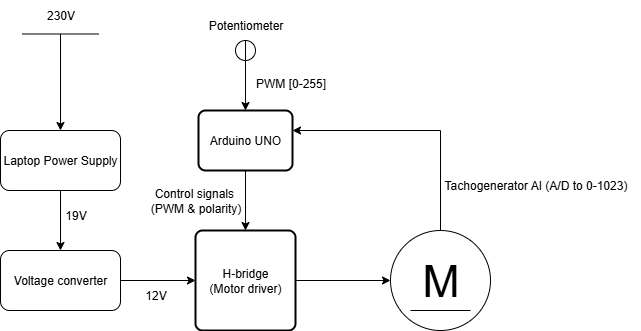
\includegraphics[width=1\textwidth,height=6cm,keepaspectratio]{motor_scheme.png}
        }

        \figcaption{ 
            Fotografia a schéma motora.
        }
        \label{fj_01_data_pot0}
    }%vbox

\end{center}

%Prechodova ----------------------------------------------------------------


\section{Prechodová charakteristika systému}

\noindent
Prechodová charakteristika predstavuje reakciu systému na jednotkový skok. Je dôležité zdôrazniť, že v tomto prípade nás zaujíma zmena vstupu, ktorá tento skok definuje – skok veľkosti 10 môže nastať z $0$ na $10$, ale rovnako aj z $20$ na $30$. V oboch prípadoch ide o jednotkový skok veľkosti 10 a pri lineárnych systémoch očakávame rovnaký tvar odozvy, len s inými číselnými hodnotami.

\medskip

\noindent
V tomto prípade analyzujeme reakciu systému na skok z hodnoty $0$ na hodnotu $30$.

\begin{center}
    \vbox{%
        \makebox[\textwidth][c]{%
        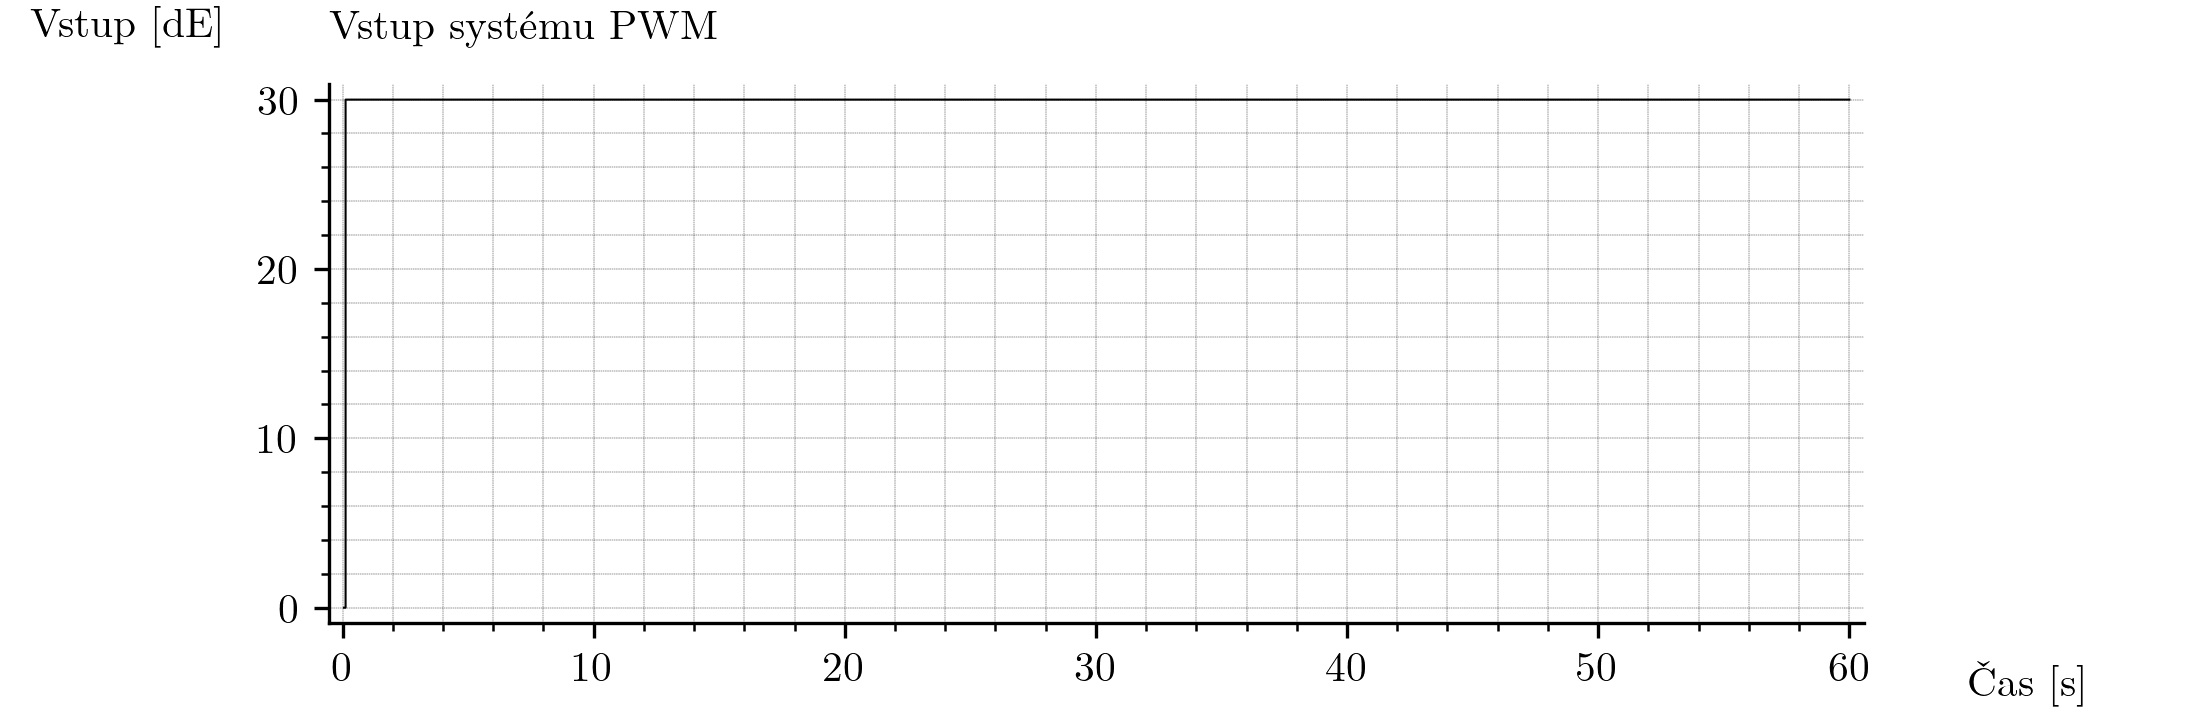
\includegraphics[width=1.4\textwidth]{prechodova_input.png}
        }

        \figcaption{ 
            Vstupný signál systému – jednotkový skok z 0 na 30 [V].
        }
        \label{fig_prechod_vstup}
    }%vbox
\end{center}

\begin{center}
    \vbox{%
        \makebox[\textwidth][c]{%
        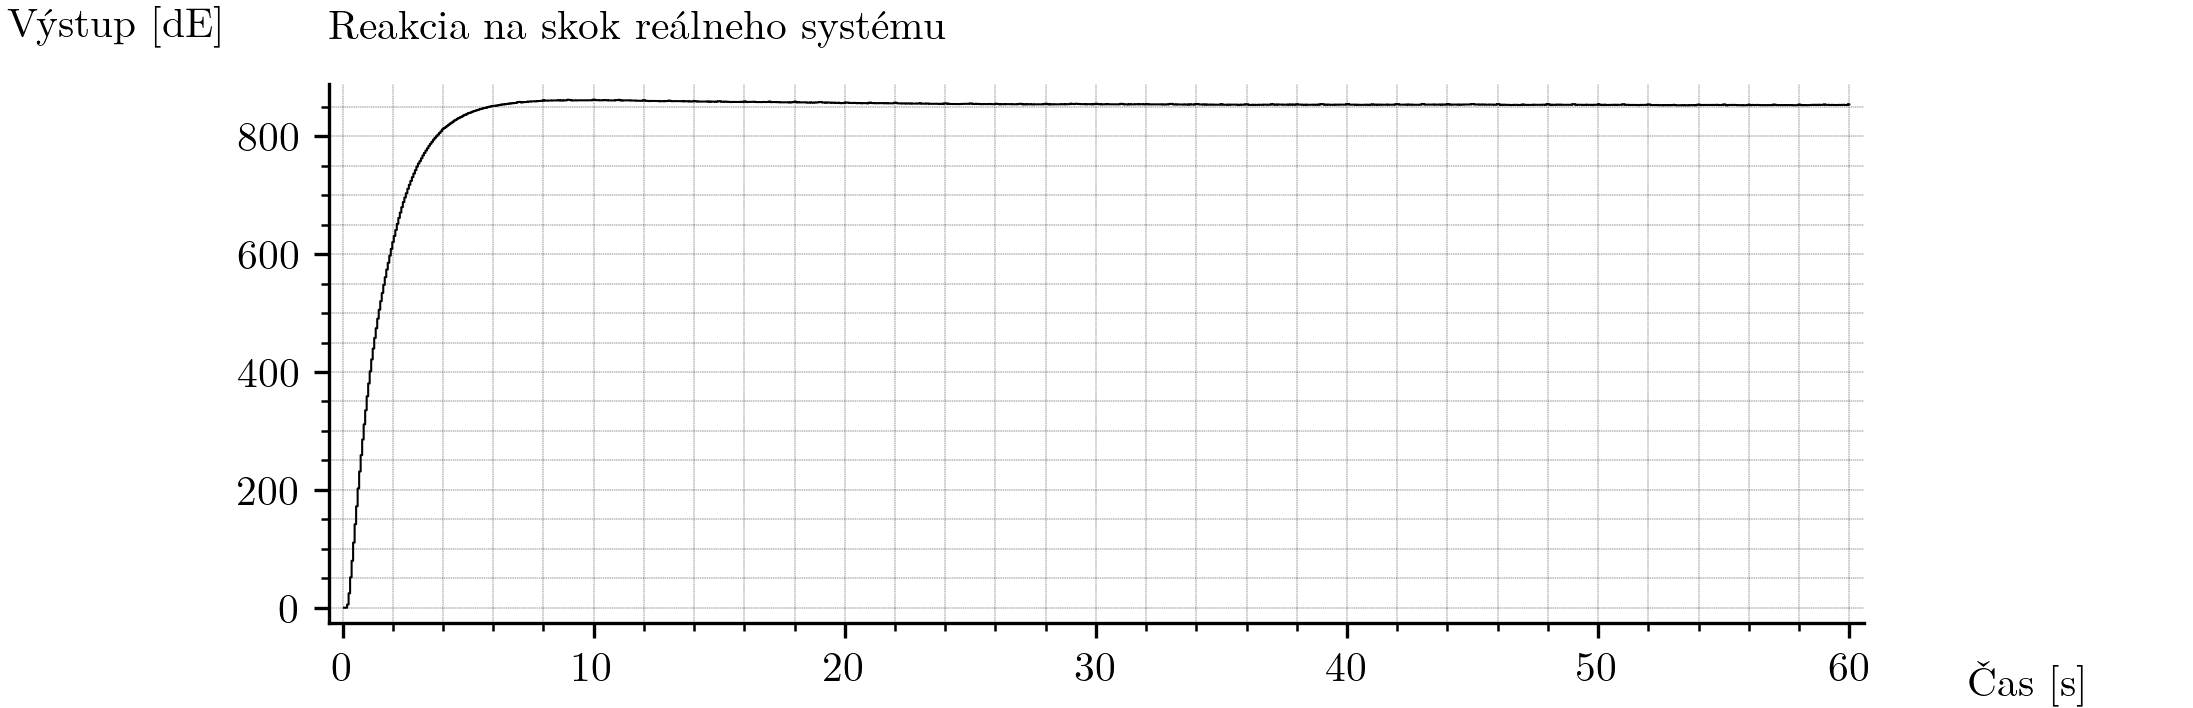
\includegraphics[width=1.4\textwidth]{prechodova_out_real.png}
        }

        \figcaption{ 
            Výstup systému ako reakcia na skokový vstup znázornený na obr.~\ref{fig_prechod_vstup}.
        }
        \label{fig_prechod_vystup}
    }%vbox
\end{center}

\noindent
Z prechodovej charakteristiky možno získať viaceré dynamické parametre systému, ako napríklad zosilnenie, čas ustálenia, odchýlku ustálenia, prekmit a ďalšie. Tieto však nie sú predmetom tejto kapitoly.

\medskip

\noindent
V ďalšom kroku pristúpime k identifikácii systému pomocou funkcie \texttt{tfest}:

\begin{lstlisting}[language=Matlab, caption=Identifikácia systému z prechodovej charakteristiky]
data = iddata(out, in, 0.06);
sys = tfest(data, 2, 1);
\end{lstlisting}

\noindent
Výsledkom je prenosová funkcia systému v tvare:

\[
G(s) = \frac{15{,}16\,s + 90{,}78}{s^2 + 4{,}83\,s + 3{,}183}
\]

\newpage

\noindent
Na základe identifikovanej prenosovej funkcie môžeme simulovať odozvu systému na rovnaký skokový vstup a porovnať ju s reálnou odozvou:

\begin{center}
    \vbox{%
        \makebox[\textwidth][c]{%
        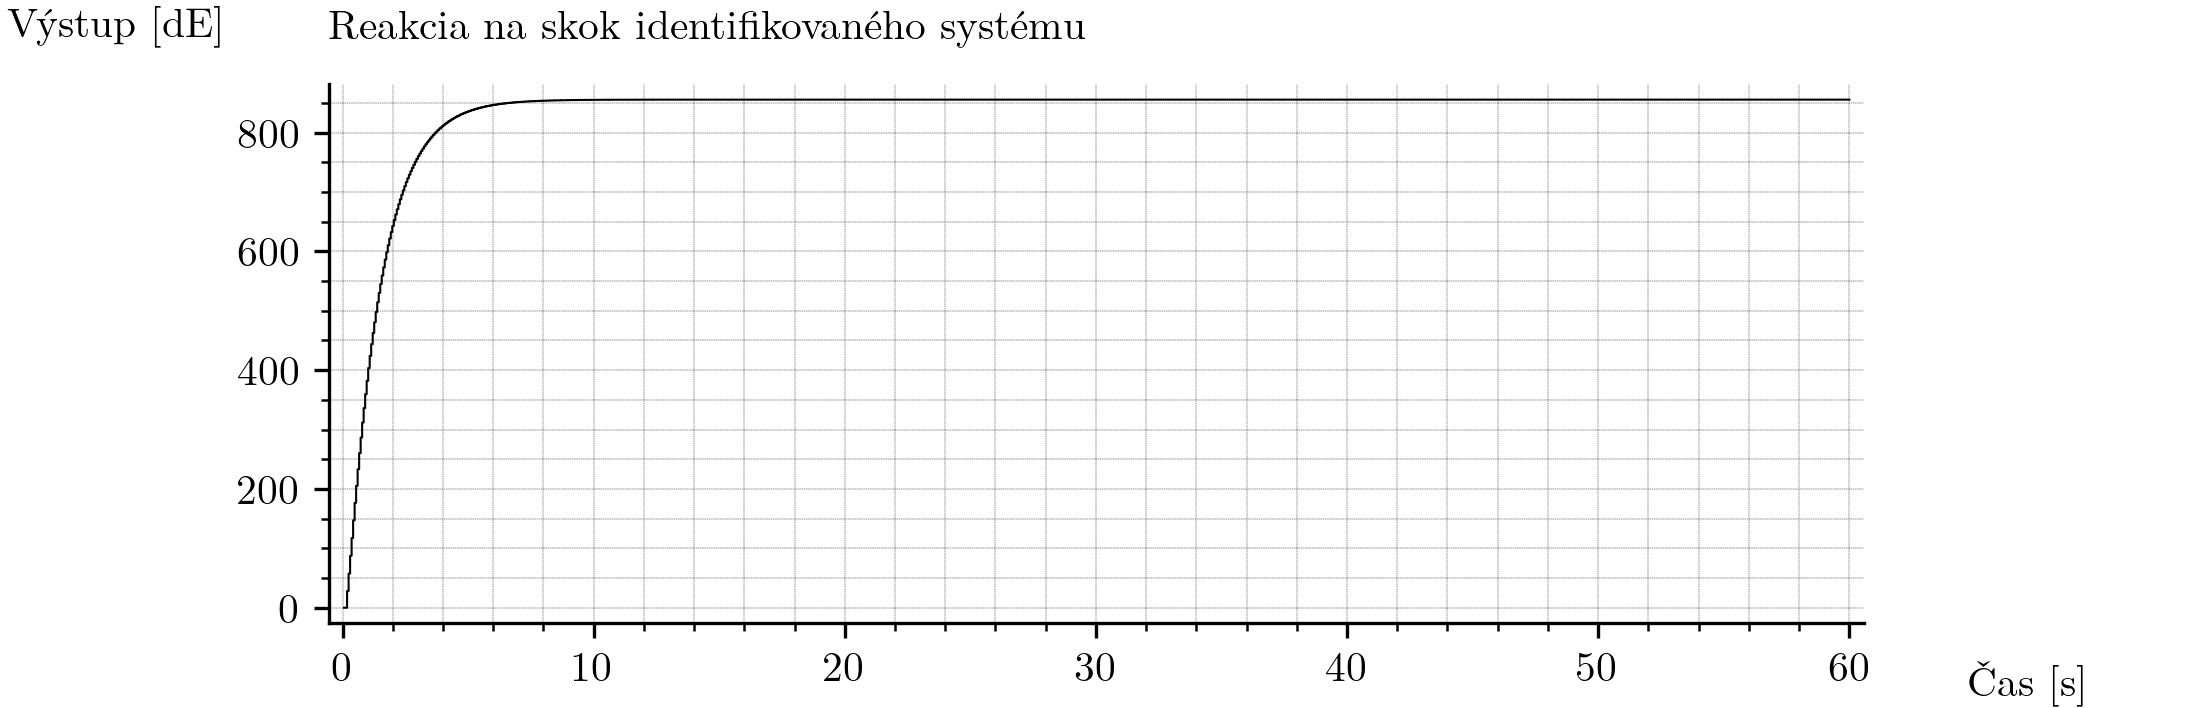
\includegraphics[width=1.4\textwidth]{prechodova_out_sim.png}
        }

        \figcaption{ 
            Simulovaná výstupná reakcia identifikovaného systému.
        }
        \label{fig_simulacia_vystup}
    }%vbox
\end{center}

\noindent
Presnosť simulácie hodnotíme pomocou strednej kvadratickej chyby (RMSE), ktorú definujeme nasledovne:

\[
\text{RMSE} = \sqrt{\frac{1}{N} \sum_{i=1}^{N} \left( y_i^\text{real} - y_i^\text{sim} \right)^2}
\]

\begin{lstlisting}[language=Matlab, caption=Výpočet strednej kvadratickej chyby]
rmse = sqrt(mean((out - out_sim).^2));
\end{lstlisting}

\noindent
Pre tento prípad platí: \textbf{RMSE = 5{,}8198}, čo predstavuje uspokojivý výsledok.

%Prevodova ----------------------------------------------------------------

\section{Statické vlastnosti: Prevodová charakteristika}

\noindent
V tejto časti sa zameriame na statické vlastnosti systému, teda určujeme, v akých ustálených bodoch sa systém nachádza pri rôznych hodnotách vstupu. 

\medskip

\noindent
Za týmto účelom sme vykonali meranie, pri ktorom sa vstup systému menil od $0$ do $255$, a to tak, že každých $20$ sekúnd sa vstup zvýšil o $2{,}5\,\%$. Celkovo bolo vykonaných 41 meraní počas doby $820$ sekúnd.

\begin{center}
    \vbox{%
        \makebox[\textwidth][c]{%
        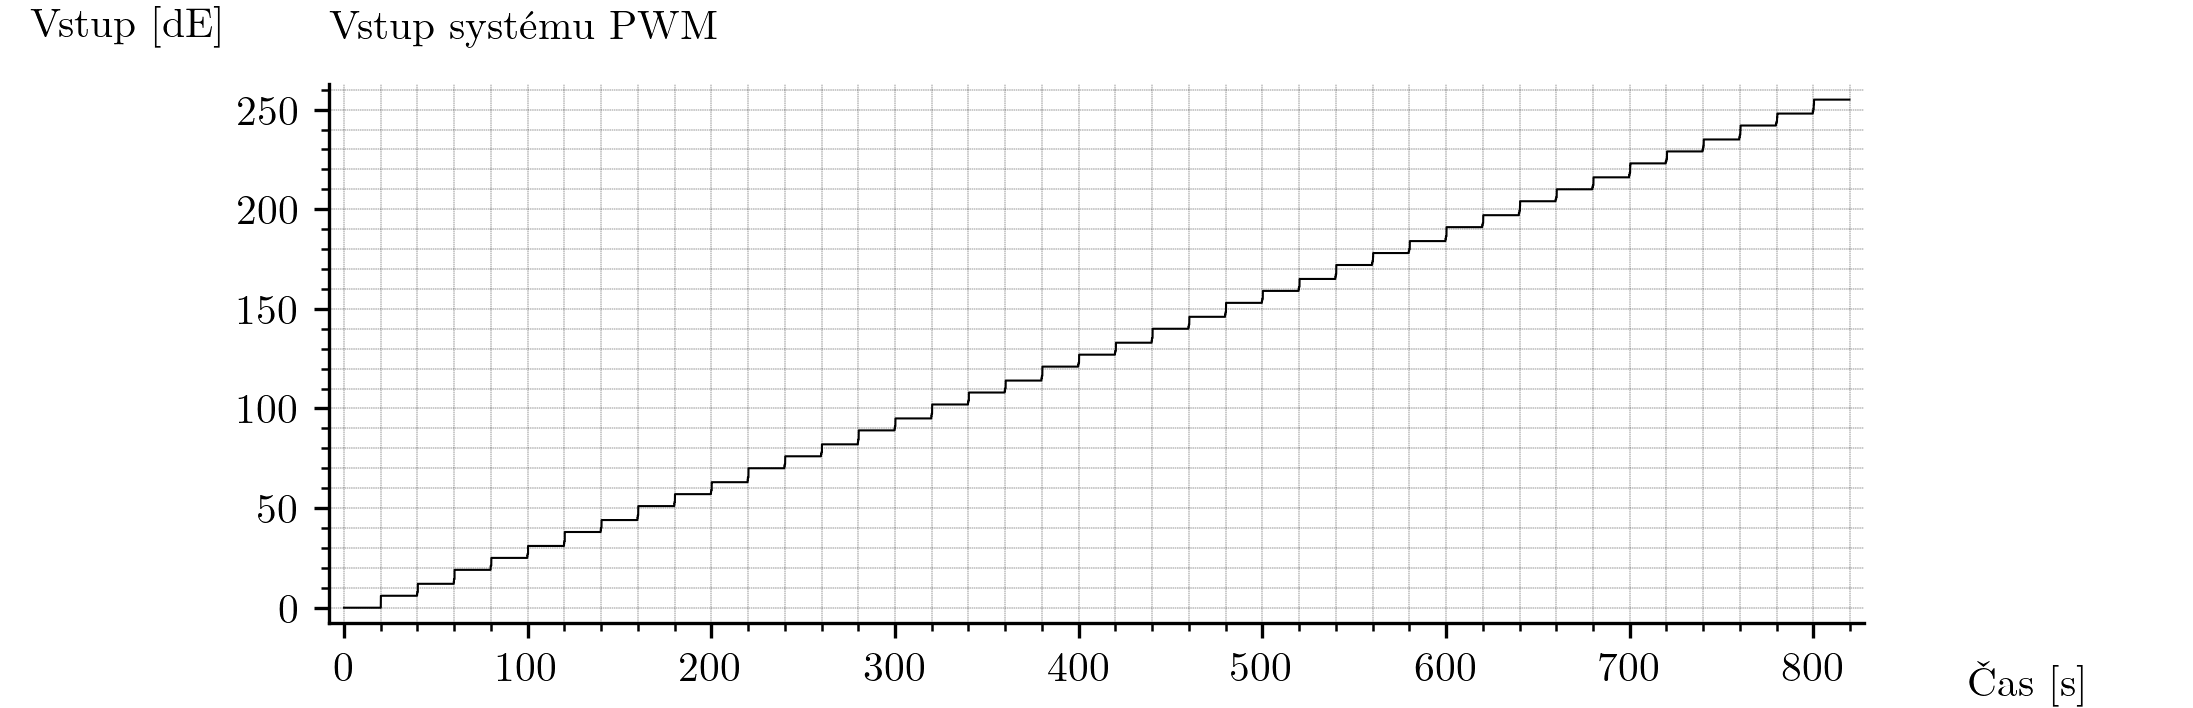
\includegraphics[width=1.4\textwidth]{prevodova_input.png}
        }

        \figcaption{ 
            Vstupný signál počas merania statickej charakteristiky.
        }
        \label{fig_staticky_vstup}
    }%vbox
\end{center}

\begin{center}
    \vbox{%
        \makebox[\textwidth][c]{%
        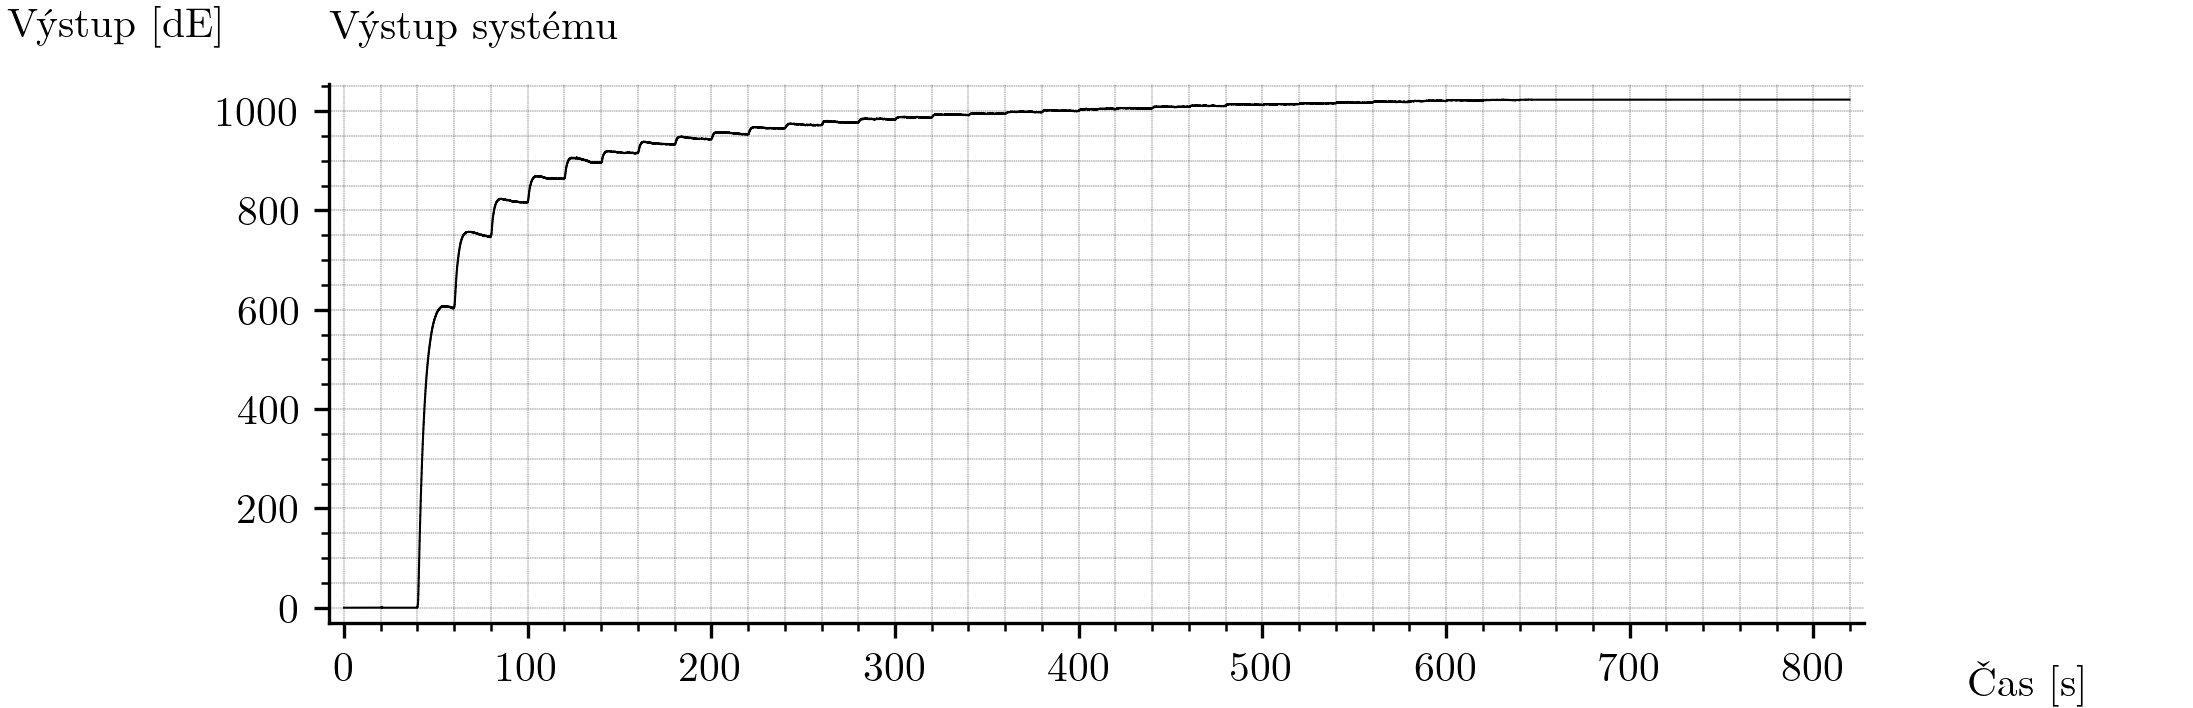
\includegraphics[width=1.4\textwidth]{prevodova_output.png}
        }

        \figcaption{ 
            Výstup systému počas merania statickej charakteristiky.
        }
        \label{fig_staticky_vystup}
    }%vbox
\end{center}

\noindent
Ako možno vidieť na výstupnom grafe (obr.~\ref{fig_staticky_vystup}), systém nie je lineárny. Nasýtenie systému nastáva veľmi rýchlo, čo výrazne komplikuje prácu s ním, keďže oblasť, v ktorej možno pozorovať dynamiku systému, je koncentrovaná len v počiatočnej časti rozsahu vstupu.

\medskip

\noindent
Na základe ustálených hodnôt vstupov a výstupov môžeme zostrojiť statickú prevodovú charakteristiku systému:

\begin{center}
    \vbox{%
        \makebox[\textwidth][c]{%
        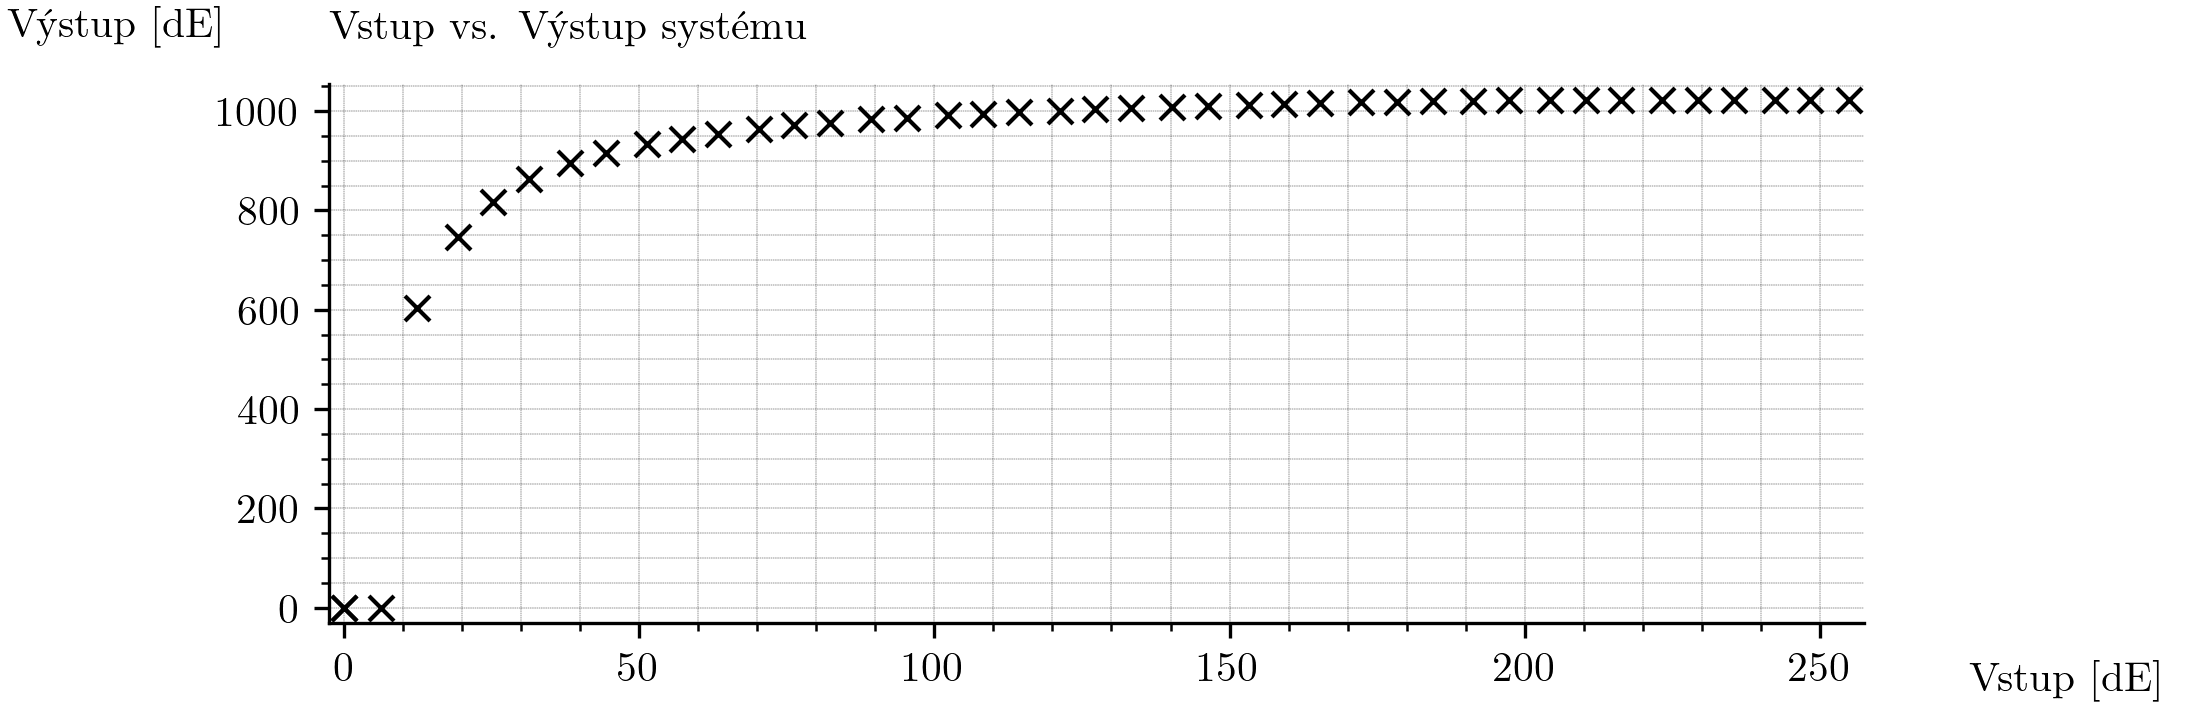
\includegraphics[width=1.4\textwidth]{prevodova_in_out.png}
        }

        \figcaption{ 
            Statická prevodová charakteristika: ustálené výstupy vzhľadom na vstup.
        }
        \label{fig_staticka_krivka}
    }%vbox
\end{center}

\noindent
Z grafu vyplýva, že identifikovať celý systém s dostatočnou presnosťou nie je možné, pretože, ako bolo spomenuté, správanie systému je výrazne nelineárne.

%Frekvencna -------------------------------------------------------------

\section{Frekvenčná charakteristika}

\noindent
V tejto časti si stručne vysvetlíme, čo je to frekvenčná charakteristika a ako ju možno určiť.

\medskip

\noindent
Ako vstup do systému sa používa harmonický signál s konkrétnou frekvenciou — v našom prípade sínusoida. Na výstupe systému očakávame signál s rovnakou frekvenciou, avšak jeho amplitúda, fázový posun, a často aj samotný tvar signálu, sa môže meniť. Práve závislosť amplitúdového zosilnenia a fázového posunu od frekvencie tvorí frekvenčnú charakteristiku systému, ktorá nás zaujíma.

\medskip

\noindent
Merania boli realizované počas 75 meracích periód, pričom každá trvala $70$ sekúnd. Celkový čas merania bol teda $5250$ sekúnd. Počas prvých $20$ sekúnd každej periódy bol na vstupe konštantný signál, aby sa systém dostal do ustáleného stavu. Následne sa počas $50$ sekúnd aplikovala sínusová funkcia s pevne danou frekvenciou.

\noindent
Použitý rozsah frekvencií bol od $0{,}02$~Hz do $1{,}5$~Hz s krokom $0{,}02$~Hz.

\begin{center}
    \vbox{%
        \makebox[\textwidth][c]{%
        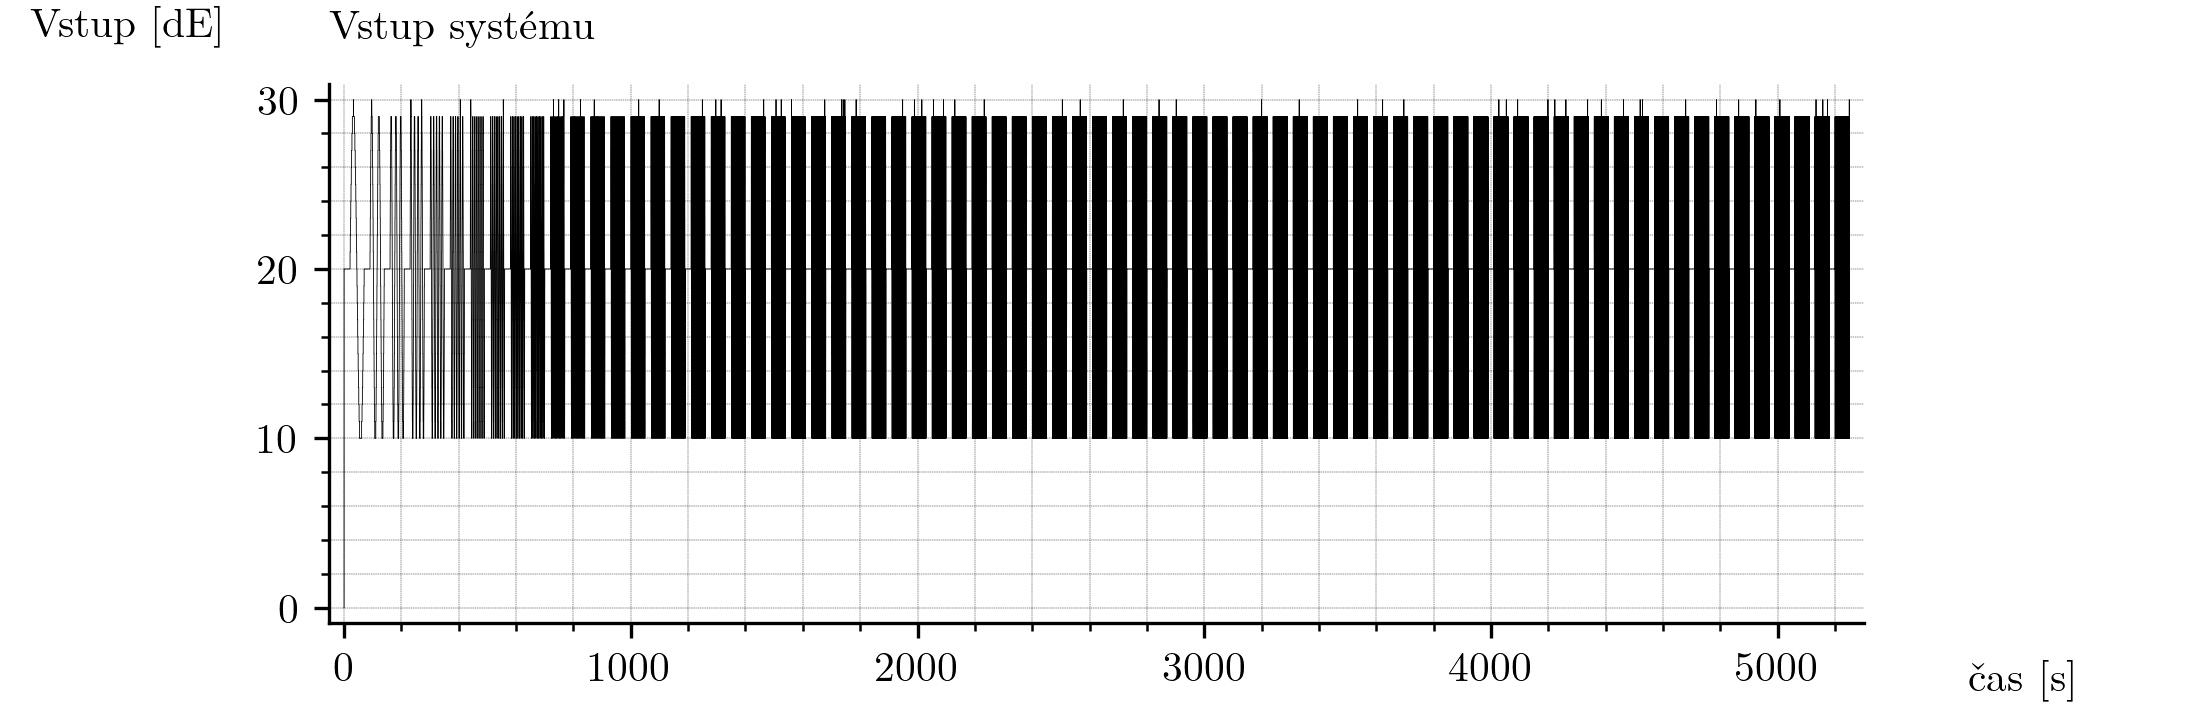
\includegraphics[width=1.4\textwidth]{frekvencna_in.png}
        }

        \figcaption{ 
            Vstupný signál systému počas frekvenčnej analýzy.
        }
        \label{fig_freq_input}
    }%vbox
\end{center}

\begin{center}
    \vbox{%
        \makebox[\textwidth][c]{%
        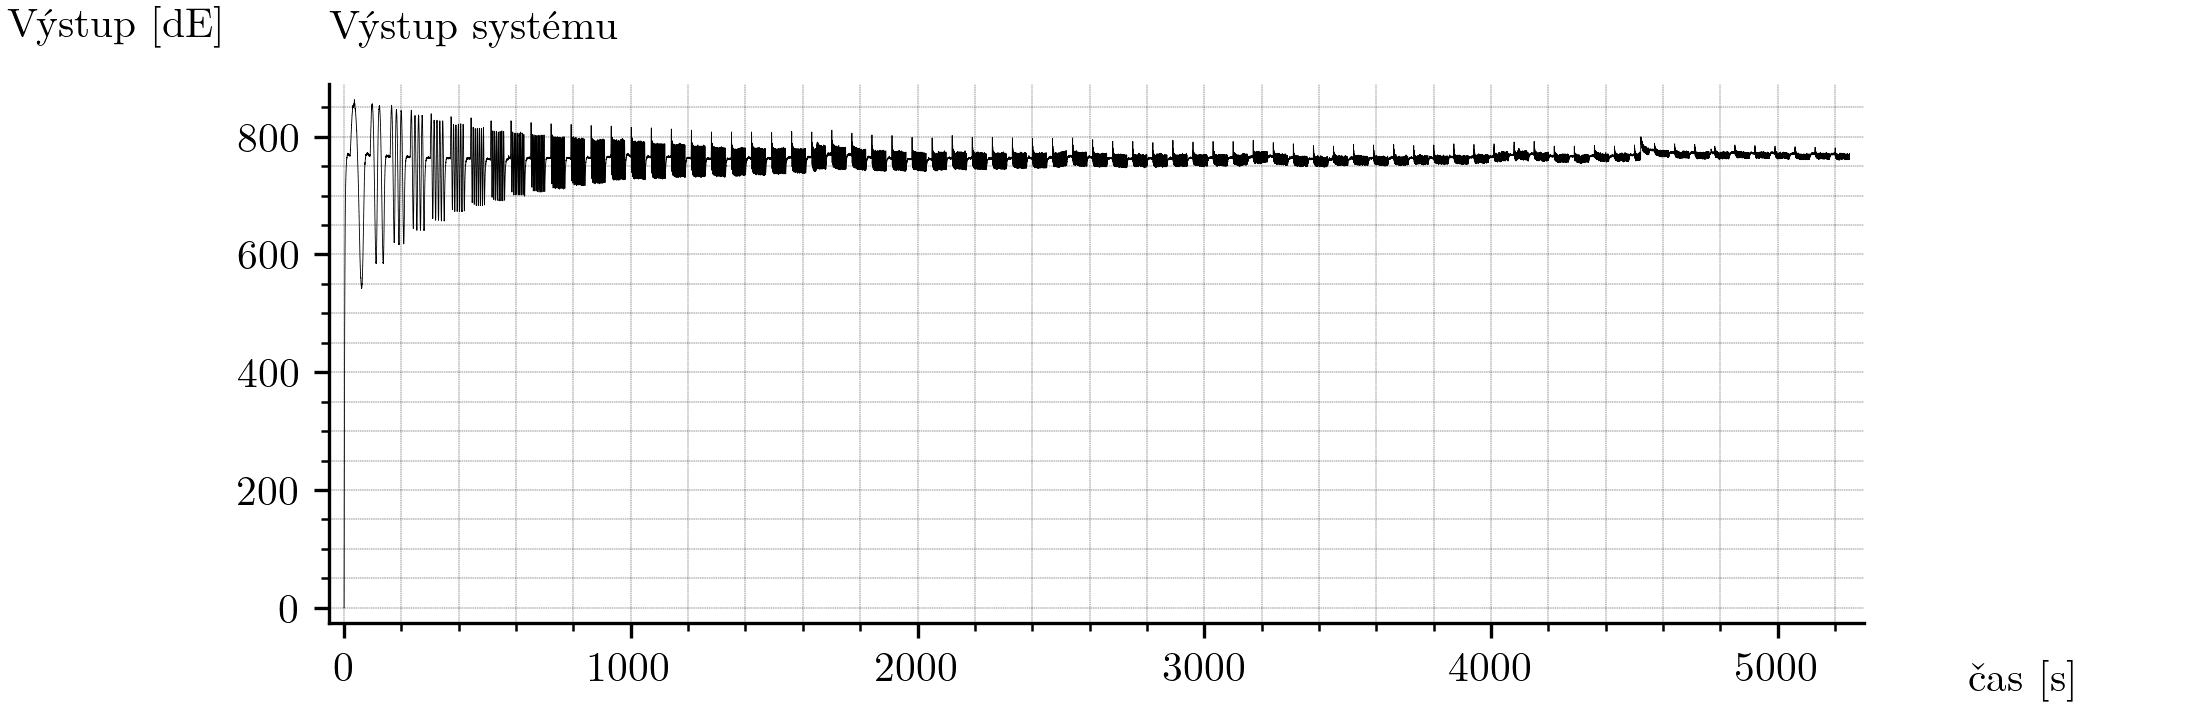
\includegraphics[width=1.4\textwidth]{frekvencna_out.png}
        }

        \figcaption{ 
            Výstupný signál systému počas frekvenčnej analýzy.
        }
        \label{fig_freq_output}
    }%vbox
\end{center}

\noindent
Pre presnejší výpočet amplitúd a fázového posunu sme pri všetkých frekvenciách okrem prvej ($0{,}02$~Hz) ignorovali prvý periodický priebeh signálu.

\subsection*{Skript na výpočet amplitúd a fázového posunu}

\begin{lstlisting}[language=Matlab, caption=Výpočet frekvenčnej charakteristiky systému]
% Frequency response calculation
for i = 1:N_freqs
    if i == 1
        f = freqs(i);
        t_start = 20 + (i - 1) * 70;    
        t_end = t_start + 50;
    else
        f = freqs(i);
        period = 1 / f;
        t_start = t_end + 20 + period;  
        t_end = t_start + (50 - period);  
    end

    idx = find(t >= t_start & t < t_end);
    t_seg = t(idx);
    u_seg = in(idx);
    y_seg = out(idx) - y0;

    omega = 2 * pi * f;
    ref_cos = cos(omega * (t_seg - t_start));
    ref_sin = sin(omega * (t_seg - t_start));

    % correlation
    U_cos = 2/length(u_seg) * sum((u_seg - mean(u_seg)) .* ref_cos);
    U_sin = 2/length(u_seg) * sum((u_seg - mean(u_seg)) .* ref_sin);
    A_in = sqrt(U_cos^2 + U_sin^2);

    Y_cos = 2/length(y_seg) * sum(y_seg .* ref_cos);
    Y_sin = 2/length(y_seg) * sum(y_seg .* ref_sin);
    A_out = sqrt(Y_cos^2 + Y_sin^2);

    amp_in(i) = A_in;
    amp_out(i) = A_out;

    phase_rad = atan2(-Y_sin, Y_cos);  
    phase_deg(i) = rad2deg(phase_rad);
end

amp = amp_out ./ amp_in;
phase_rad = deg2rad(phase_deg);
log_freqs = log10(freqs);
\end{lstlisting}

\subsection*{Popis výpočtu}

\noindent
Skript rozdeľuje signál na segmenty podľa jednotlivých frekvencií a pomocou korelácie s referenčnými sínusovými a kosínusovými signálmi odhaduje amplitúdu a fázový posun pre vstup aj výstup. Výsledkom sú vektory amplitúdového zosilnenia a fázového posunu ako funkcie frekvencie.

\begin{center}
    \vbox{%
        \makebox[\textwidth][c]{%
        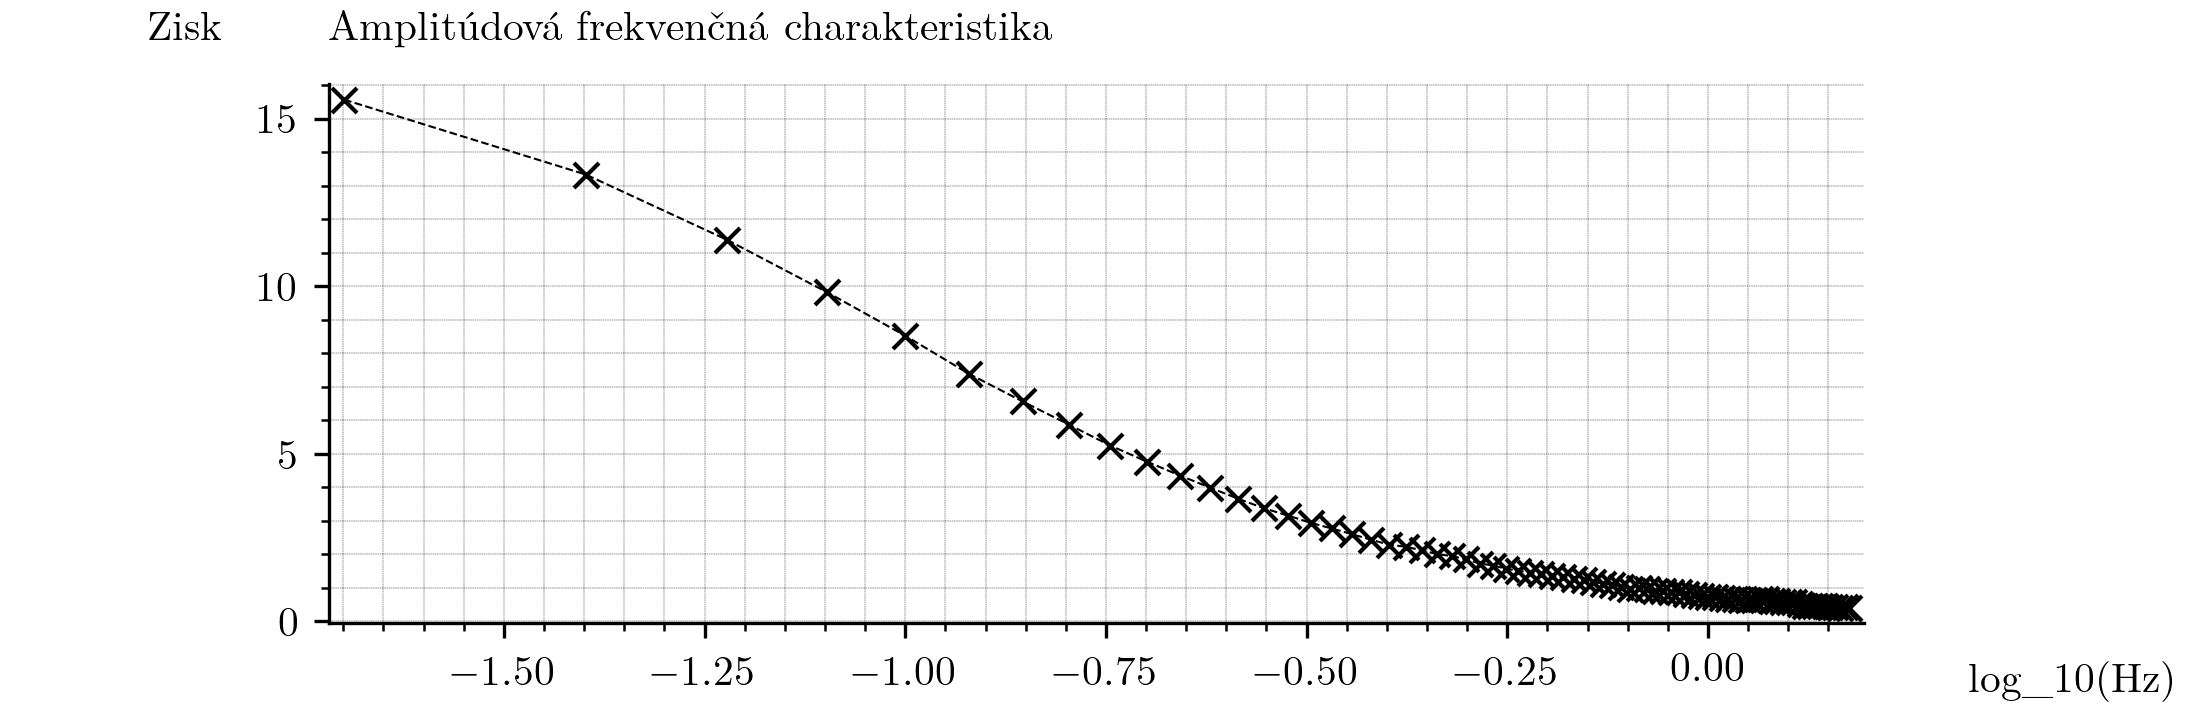
\includegraphics[width=1.4\textwidth]{frekvencna_amp.png}
        }

        \figcaption{ 
            Amplitúdová charakteristika systému (závislosť zisku od frekvencie).
        }
        \label{fig_amp_gain}
    }%vbox
\end{center}

\begin{center}
    \vbox{%
        \makebox[\textwidth][c]{%
        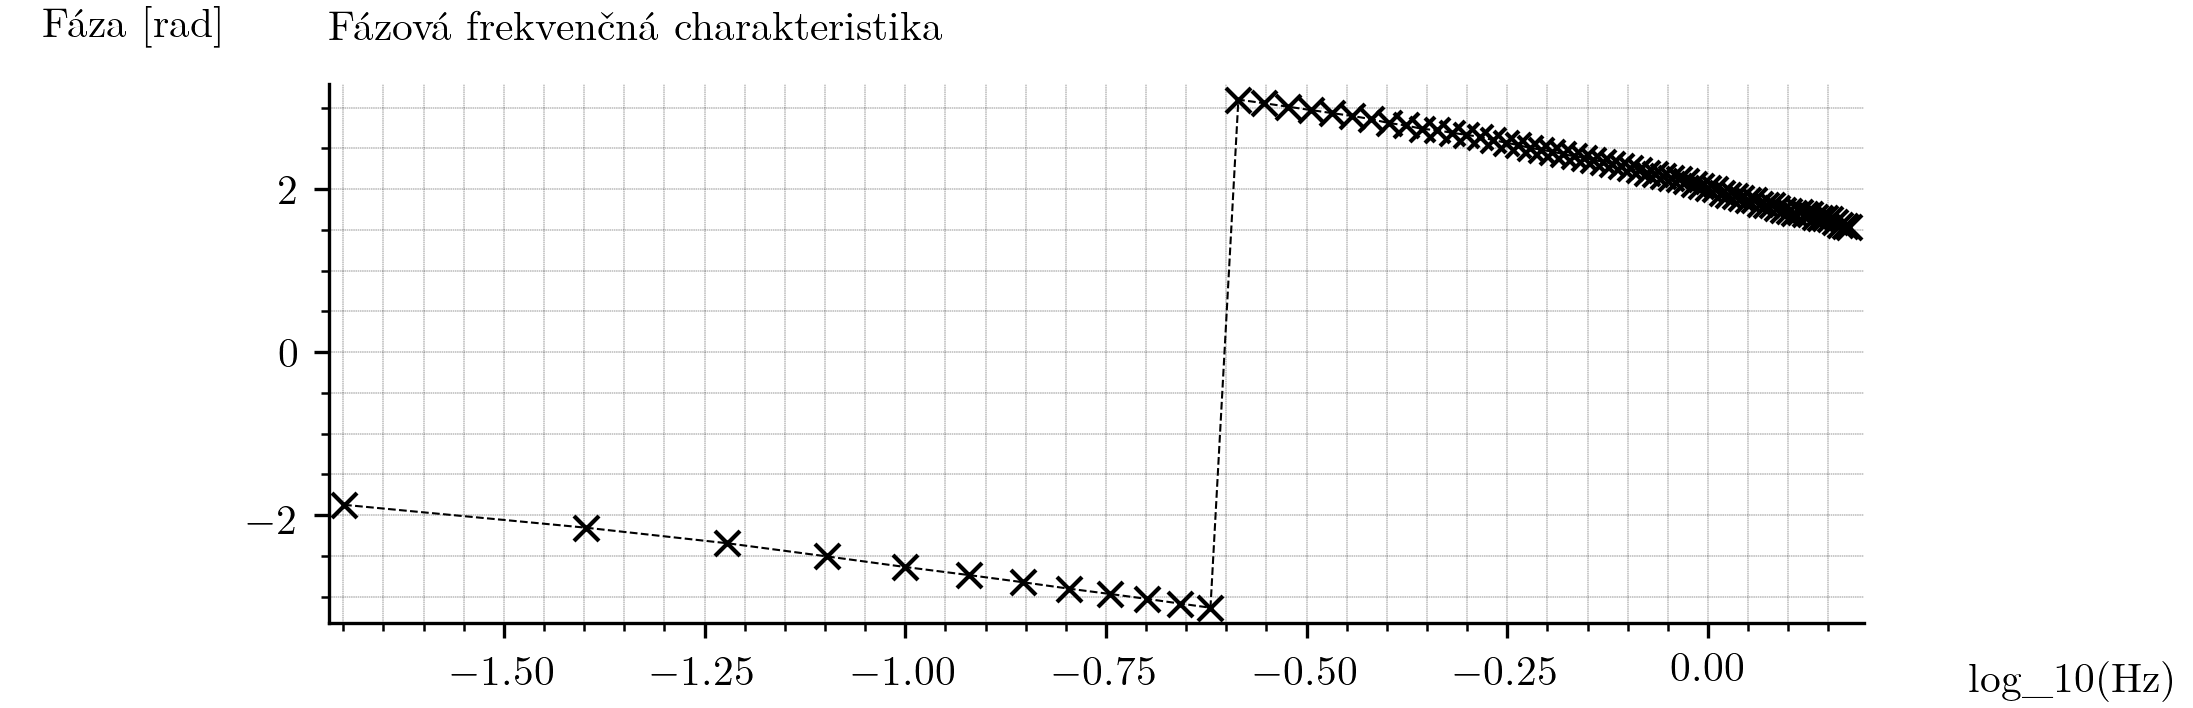
\includegraphics[width=1.4\textwidth]{frekvencna_phase.png}
        }

        \figcaption{ 
            Fázová charakteristika systému (závislosť fázového posunu od frekvencie).
        }
        \label{fig_phase_shift}
    }%vbox
\end{center}

\noindent
Na základe tejto frekvenčnej charakteristiky je možné podniknúť konkrétne kroky na potlačenie rezonancií, zníženie fázového posunu a zlepšenie správania systému vo frekvenčnej oblasti.







% -----------------------------------------------------------------------------

\end{document}

% -----------------------------------------------------------------------------